%% pyRMT method paper -- Elsevier (elsarticle) format.
%% Primary target: Journal of Computational Physics. Fallback: Computers & Fluids.
%% Build:  pdflatex main ; bibtex main ; pdflatex main ; pdflatex main
\documentclass[review,3p,11pt]{elsarticle}

\usepackage{amsmath,amssymb,bm}
\usepackage{amsthm}
\usepackage{mathtools}
\usepackage{graphicx}
\usepackage{booktabs}
\usepackage{enumitem}
\usepackage[hidelinks]{hyperref}
\usepackage{cleveref}
\usepackage{xcolor}

\newtheorem{proposition}{Proposition}
\theoremstyle{remark}
\newtheorem{remark}{Remark}

% placeholder figure box (draft only): \phfig{label}{caption}
\newcommand{\phfig}[2]{%
  \begin{figure}[t]\centering
  \fbox{\parbox[c][0.28\textheight][c]{0.72\textwidth}{\centering
    \color{blue}\texttt{[figure placeholder: #1]}}}
  \caption{#2}\label{#1}
  \end{figure}}

% ---- draft placeholder macro (remove for submission) ----
\newcommand{\TODO}[1]{{\color{red}\textbf{[TODO: #1]}}}
\newcommand{\PLACE}[1]{{\color{blue}\texttt{<#1>}}}

% ---- notation ----
\newcommand{\uv}{\bm{u}}                 % velocity
\newcommand{\xv}{\bm{x}}                 % Eulerian position
\newcommand{\Xv}{\bm{X}}                 % reference position
\newcommand{\xiv}{\bm{\xi}}              % reference map
\newcommand{\Ften}{\bm{F}}              % deformation gradient
\newcommand{\bt}{\bm{b}}                 % left Cauchy-Green / Finger
\newcommand{\be}{\bm{b}_e}              % elastic Finger tensor
\newcommand{\Lt}{\bm{L}}                % velocity gradient
\newcommand{\It}{\bm{I}}                % identity
\newcommand{\sig}{\bm{\sigma}}          % Cauchy stress
\newcommand{\psib}{\bm{\psi}}           % log-conformation psi = log b_e
\newcommand{\grad}{\nabla}
\newcommand{\dive}{\grad\!\cdot\!}
\newcommand{\dt}{\Delta t}
\newcommand{\dx}{\Delta x}
\newcommand{\Dt}[1]{\tfrac{D #1}{D t}}
\newcommand{\tr}{\operatorname{tr}}
\newcommand{\dev}{\operatorname{dev}}

\journal{Journal of Computational Physics}

\begin{document}

\begin{frontmatter}

\title{An implicit, monolithic, incompressible Reference Map Technique for
viscoelastic fluid--structure interaction}

\author[a]{Saman Seifi\corref{cor}}
\cortext[cor]{Corresponding author}
\affiliation[a]{organization={Affiliation TODO}, country={Country TODO}}

\begin{abstract}
We present a fully Eulerian, one-fluid Reference Map Technique (RMT) for
incompressible fluid--structure interaction (FSI) that couples a finite-strain
\emph{viscoelastic} solid to a Newtonian fluid on a single staggered (MAC) grid with one
pressure solve. The method differs from existing Eulerian FSI in two ways. First, the
stress-carrying strain is transported as a log-conformation tensor $\psib=\log\be$
(Fattal--Kupferman; Hulsen \emph{et al.}), which is positive-definite by construction and
decouples the relaxing elastic stress from the folding-prone reference map; monolithic,
implicit Eulerian FSI has been demonstrated for hyperelastic solids
\cite{Richter2013,Dunne2006} but not, to our knowledge, for a finite-strain viscoelastic
solid. Second, we develop the time integration as a stack that lifts the stiff time-step
limits: an implicit--explicit (IMEX) scheme---backward-Euler viscosity via the pressure
transforms, exact exponential relaxation, an energy-conserving trapezoidal elastic
coupling, and adaptive semi-Lagrangian advection---removes the viscous, relaxation,
elastic-wave and advective CFL restrictions in a fractional-step setting; and a
Jacobian-free Newton--Krylov (JFNK) formulation solves the coupled
$(\uv,p,\xiv,\psib)$ system \emph{monolithically}, with the reference map a coupled unknown
(the step \cite{Richter2013} lags), preconditioned by the split IMEX solver and the exact
projection. The staggered discretization makes the projection exact (machine-zero
divergence). We verify the constitutive update against analytic viscometric limits to
machine precision, confirm the exact projection and spatial order on manufactured and
Taylor--Green problems, and
validate the coupled solver against the Ghia lid-driven cavity and the Sugiyama soft-disc
benchmark. The trapezoidal elastic coupling is energy-conserving on a standing elastic
wave, and a DST-preconditioned solve keeps the wall-bounded Helmholtz at a few iterations
independent of resolution. On the soft-disc benchmark the semi-Lagrangian IMEX scheme runs
stably at several times the explicit step (e.g.\ $6\times$ in $\sim\!4\times$ fewer steps),
at a modest, controllable accuracy cost that the monolithic JFNK solve removes by treating
advection and the elastic coupling implicitly and consistently. We report a work--precision
comparison across the explicit, IMEX and monolithic integrators and delineate the regimes
(stiff solids, high Weissenberg) where implicit integration pays off.
\end{abstract}

\begin{keyword}
reference map technique \sep fluid--structure interaction \sep viscoelasticity \sep
log-conformation \sep implicit time integration \sep Eulerian solid mechanics
\end{keyword}

\end{frontmatter}

\section{Introduction}
\label{sec:intro}

Fully Eulerian formulations of fluid--structure interaction (FSI) discretize the
solid and the fluid on a single fixed grid, sharing one velocity field and one
pressure solve. This removes the mesh-conforming remeshing and the partitioned
added-mass instabilities of arbitrary Lagrangian--Eulerian and immersed-boundary
approaches, at the price of representing the finite-strain solid response in the
laboratory frame. The \emph{reference map technique} (RMT) does so by transporting
the inverse motion---the reference map $\xiv(\xv,t)$ mapping a current point back to
its material label---from which the deformation gradient and hence the elastic stress
are reconstructed \cite{Kamrin2012,Valkov2015}. The RMT has been developed into a
robust incompressible FSI method \cite{Rycroft2020} and a conservative, non-dissipative
finite-difference formulation \cite{Jain2019}.

Three limitations of the existing RMT literature motivate this work.
\begin{enumerate}[label=(\roman*),nosep]
\item \textbf{The solid is hyperelastic.} A purely hyperelastic solid sheared without
bound stores unbounded energy; the reference map then folds, and reinitialization
treats the symptom rather than the cause. A relaxing (viscoelastic) stress is the
principled remedy, but it must not reintroduce the loss of positive-definiteness that
plagues conformation-tensor transport.
\item \textbf{The time integration is explicit.} The dominant RMT formulations
\cite{Kamrin2012,Rycroft2020,Jain2019} advance momentum explicitly, so the time step
is throttled by the elastic-wave speed $c_s=\sqrt{\mu_s/\rho}$, the viscous diffusion
$\dx^2/\nu$, and---for a viscoelastic solid---the relaxation time $\tau$. Stiff solids
and high-Weissenberg regimes are effectively out of reach.
\item \textbf{Unified Eulerian alternatives are compressible.} The Godunov--Peshkov--%
Romenski (GPR) model unifies viscous fluids and elastoplastic/viscoelastic solids in a
single first-order hyperbolic system \cite{Peshkov2016,Dumbser2016}, but it is
compressible and advanced with explicit or semi-implicit high-order schemes; an
\emph{implicit, monolithic, incompressible} treatment remains an open gap.
\end{enumerate}

\paragraph{Contributions.} We address all three within one collocated-velocity,
one-pressure RMT:
\begin{enumerate}[label=(\arabic*),nosep]
\item A finite-strain viscoelastic solid whose stress-carrying strain is transported as
the \emph{log-conformation} tensor $\psib=\log\be$ \cite{Fattal2004}, guaranteeing
$\be\succ0$ by construction and decoupling the relaxing stress from the folding-prone
reference map. The standard-linear-solid form retains an equilibrium hyperelastic
branch so the body still returns to shape; $\tau\to\infty$ recovers neo-Hookean RMT.
\item An implicit--explicit (IMEX) time-integration \emph{stack} that lifts the stiff
CFL limits one term at a time---backward-Euler viscosity through the pressure
transform/Krylov solvers, exact exponential relaxation, and a linearly-implicit
elastic-wave stabilizer---culminating in
\item a fully-implicit, monolithic Newton--Krylov solve of the coupled
$(\uv,p,\xiv,\psib)$ system that lifts the elastic-wave CFL while retaining accuracy,
reusing the exact pressure projection as the saddle-point preconditioner.
\end{enumerate}
The staggered (MAC) discretization renders the projection exact
(machine-zero divergence), removing the checkerboard/Rhie--Chow workarounds of the
collocated formulation. \Cref{sec:governing,sec:rmt,sec:constitutive} set out the
continuous model, \cref{sec:discretization,sec:time} the discretization and the
IMEX/monolithic time integration, and \cref{sec:verification,sec:validation,sec:results}
the verification, validation, and performance results.

\section{Governing equations}
\label{sec:governing}

We consider an incompressible medium on a fixed domain $\Omega\subset\mathbb{R}^2$
occupied by a Newtonian fluid and one or more finite-strain solid bodies. A single
velocity field $\uv(\xv,t)$ and pressure $p(\xv,t)$ are shared by both phases. Momentum
and incompressibility read
\begin{align}
\rho\left(\partial_t\uv + (\uv\!\cdot\!\grad)\uv\right)
   &= -\grad p + \dive\sig_{\mathrm{d}} + \bm f_{\Gamma} + \bm f_{c},
   \label{eq:mom}\\
\dive\uv &= 0,
   \label{eq:incomp}
\end{align}
where $\rho$ is the (piecewise-constant) density, $\bm f_\Gamma$ is the surface-tension
force and $\bm f_c$ the contact force. The deviatoric stress $\sig_{\mathrm d}$ is
blended between fluid and solid through a smoothed indicator (one-fluid model),
\begin{equation}
\sig_{\mathrm d} = 2\mu_f\,\bm D
   + (1-H)\,\sig_{\!s},
   \qquad
\bm D=\tfrac12\!\left(\grad\uv+\grad\uv^{\!\top}\right),
   \label{eq:blend}
\end{equation}
with $\mu_f$ the fluid viscosity, $\bm D$ the rate-of-strain, $\sig_{\!s}$ the solid
Cauchy stress (\cref{sec:rmt,sec:constitutive}), and $H\in[0,1]$ a smoothed Heaviside
of the level set $\phi$ ($H\to1$ in the fluid, $H\to0$ in the solid). The trace of
$\sig_{\!s}$ is carried by the pressure, so only its deviatoric part enters
\cref{eq:mom} up to a redefinition of $p$.

The material occupied by the solid is tracked by the reference map (\cref{sec:rmt}),
from which the level set $\phi$ and the deformation are reconstructed. Boundary
conditions are problem-dependent (no-slip walls with an optional moving lid, free-slip
impermeable walls, or periodic); the pressure boundary condition is chosen consistently
with the velocity boundary condition (\cref{sec:discretization}).

\section{The reference map and the elastic solid}
\label{sec:rmt}

\subsection{Reference map and deformation gradient}
Let $\bm\chi(\Xv,t)$ be the motion carrying a material label $\Xv$ to its current
position $\xv$. The \emph{reference map} is the inverse,
$\xiv(\xv,t)=\bm\chi^{-1}(\xv,t)$, so $\xiv(\xv,0)=\xv$ in the solid. Because $\xiv$
labels material, it is advected passively,
\begin{equation}
\partial_t\xiv + (\uv\!\cdot\!\grad)\xiv = \bm 0 .
\label{eq:xi-advect}
\end{equation}
The deformation gradient $\Ften=\partial\xv/\partial\Xv$ is recovered in the Eulerian
frame from the spatial gradient of the reference map,
\begin{equation}
\Ften = (\grad\xiv)^{-1},
\qquad J=\det\Ften ,
\label{eq:F}
\end{equation}

\phfig{fig:rmt-schematic}{Reference map technique. \TODO{schematic: (left) material body
with label field $\Xv$ in the reference configuration; (centre) the motion $\bm\chi$ and
its inverse, the reference map $\xiv=\bm\chi^{-1}$, on the fixed Eulerian grid; (right)
$\Ften=(\grad\xiv)^{-1}$ and the solid/fluid blend across the smoothed interface $\phi$.
Draw as inline TikZ or a vector figure.}}
and the left Cauchy--Green (Finger) tensor is $\bt=\Ften\Ften^{\!\top}$. For an
incompressible motion $J\equiv1$; the discrete $J$ is monitored as a folding/quality
diagnostic.

\subsection{Neo-Hookean solid}
The equilibrium (non-relaxing) branch of the solid is an incompressible neo-Hookean
material,
\begin{equation}
\sig_{\!s}^{\infty} = \mu_s\,\dev\!\left(\Ften\Ften^{\!\top}\right)
   = \mu_s\!\left(\bt - \tfrac12\tr(\bt)\,\It\right)\quad(\text{2-D}),
\label{eq:neohookean}
\end{equation}
with shear modulus $\mu_s$ and elastic wave speed $c_s=\sqrt{\mu_s/\rho}$. In the purely
hyperelastic limit ($\tau\to\infty$, \cref{sec:constitutive}) this is the entire solid
stress; the general viscoelastic solid adds a relaxing branch.

\subsection{Level set, extrapolation, reinitialization}
The solid occupies $\{\phi\le0\}$. The level set is reconstructed from the reference map
each step (the material boundary is the image of the initial boundary under $\xiv$), and
the reference map is extrapolated into a narrow band outside the solid so that the
gradient in \cref{eq:F} and the interfacial forces have valid stencils. Optional
level-set reinitialization (PDE or fast-marching) restores a signed-distance band. The
advection of \cref{eq:xi-advect} is discretized by a switchable scheme (semi-Lagrangian
RK4 backtrace by default; central/WENO or a conservative flux form for
differentiability, \cref{sec:time}).

\section{Finite-strain viscoelasticity via log-conformation}
\label{sec:constitutive}

\subsection{Standard-linear-solid model}
The solid stress is split into a non-relaxing (equilibrium) neo-Hookean branch
\cref{eq:neohookean} and a relaxing Maxwell branch carried by an elastic Finger tensor
$\be$,
\begin{equation}
\sig_{\!s} = \mu_s\,\dev\!\left(\Ften\Ften^{\!\top}\right)
   + G\,\dev(\be),
\label{eq:sls}
\end{equation}
where $G$ is the viscoelastic modulus. The elastic Finger tensor evolves by the
upper-convected Maxwell (UCM) equation with relaxation time $\tau$,
\begin{equation}
\Dt{\be} - \Lt\be - \be\Lt^{\!\top} = -\frac1\tau\left(\be-\It\right),
\qquad \Lt=\grad\uv,
\label{eq:ucm}
\end{equation}
with $\tfrac{D}{Dt}=\partial_t+(\uv\!\cdot\!\grad)$. Dropping the equilibrium branch
($\mu_s=0$) gives a Maxwell fluid; $\tau\to\infty$ gives a purely elastic solid for
which \cref{eq:ucm} reduces to $\Dt{\be}=\Lt\be+\be\Lt^{\!\top}$, i.e.\ $\be$ tracks
$\Ften\Ften^{\!\top}$ and \cref{eq:sls} returns the neo-Hookean stress. The model
therefore spans, under one framework, elastic solid $\leftrightarrow$ viscoelastic
solid $\leftrightarrow$ viscoelastic fluid.

\paragraph{Viscometric limits (used for verification).} For homogeneous simple shear
$\Lt=\dot\gamma\,\bm e_x\!\otimes\!\bm e_y$ the steady solution of \cref{eq:ucm} is
$b_e^{xy}=\tau\dot\gamma$, $b_e^{xx}=1+2\tau^2\dot\gamma^2$, $b_e^{yy}=1$, giving
$\sigma_{xy}=G\tau\dot\gamma$ and first normal-stress difference
$N_1=2G\tau^2\dot\gamma^2$. For a step shear strain $\gamma$ held from $t=0$,
$b_e^{xy}(t)=\gamma\,e^{-t/\tau}$; for uniform planar extension at rate $\varepsilon$
with $\mathrm{Wi}=\varepsilon\tau<\tfrac12$, $b_e^{xx}\to1/(1-2\mathrm{Wi})$.

\subsection{Log-conformation transport}
Direct transport of $\be$ is either over-diffusive or, if non-dissipative, loses
positive-definiteness and blows up at high Weissenberg number. Following
Fattal--Kupferman \cite{Fattal2004} we evolve
\begin{equation}
\psib=\log\be, \qquad \be=\exp\psib\succ0\ \text{by construction.}
\label{eq:psi}
\end{equation}
Advection of $\psib$ is passive as in \cref{eq:xi-advect}; the local (homogeneous) part
of \cref{eq:ucm} is transformed to $\psib$ as follows. In the eigenframe of $\psib$
(equivalently of $\be$), with eigenvalues $\lambda_i=e^{\ell_i}$ of $\be$ and
$\bm M=\bm R^{\!\top}\Lt\bm R$ the velocity gradient rotated into that frame, the local
evolution of $\psib$ is
\begin{equation}
\dot{\psib}\big|_{\mathrm{eig}}
   = \begin{bmatrix} 2M_{11} + \tfrac1\tau(e^{-\ell_1}-1) & \Omega_{12}\\[2pt]
       \Omega_{12} & 2M_{22} + \tfrac1\tau(e^{-\ell_2}-1)\end{bmatrix},
\quad
\Omega_{12}=\frac{\ell_2-\ell_1}{\lambda_2-\lambda_1}\left(\lambda_2 M_{12}+\lambda_1 M_{21}\right),
\label{eq:logconf-rhs}
\end{equation}
rotated back by $\bm R(\cdot)\bm R^{\!\top}$; the diagonal carries stretching and
relaxation, the off-diagonal the eigenvector rotation. The degenerate limit
$\ell_1\!\to\!\ell_2$ of $\Omega_{12}$ is $e^{-\ell_1}(M_{12}+M_{21})$, recovering
$\dot{\psib}=2\,\mathrm{sym}(\Lt)$ at $\be=\It$, so \cref{eq:logconf-rhs} is smooth.
In two dimensions the eigendecomposition of the symmetric $2\times2$ field is available
in closed form, so \cref{eq:logconf-rhs} is evaluated without iterative diagonalization.

\subsection{Exact relaxation for stiff \texorpdfstring{$\tau$}{tau}}
\label{sec:exact-relax}
The relaxation term $-\tfrac1\tau(\be-\It)$ is stiff for small $\tau$ (high
Weissenberg), forcing $\dt\lesssim\tau$ under explicit integration. We remove this by
Strang-splitting the local update into
$\text{relax}(\dt/2)\!\to\!\text{stretch}(\dt)\!\to\!\text{relax}(\dt/2)$ and
integrating the relaxation substep \emph{analytically}. The relaxation-only equation
$\dot{\be}=-\tfrac1\tau(\be-\It)$ has the exact solution
\begin{equation}
\be \leftarrow \It + (\be-\It)\,e^{-\dt/\tau},
\label{eq:relax-exact}
\end{equation}
which is unconditionally stable for any $\tau$ and positive-definite-preserving, since
\cref{eq:relax-exact} is the convex combination $(1-e^{-\dt/\tau})\It+e^{-\dt/\tau}\be$
of two SPD tensors. The stretch substep uses \cref{eq:logconf-rhs} with $\tau\to\infty$
(explicit, non-stiff, bounded by the velocity-gradient magnitude). For a step strain
this scheme is exact at any $\dt$; the property is verified in \cref{sec:verification}.

\section{Spatial discretization and exact projection}
\label{sec:discretization}

\subsection{Staggered (MAC) grid}
The domain $[0,L_x]\times[0,L_y]$ is divided into $N_x\times N_y$ cells of size
$\dx\times\Delta y$. Pressure and the reference map live at cell centres,
$x$-velocity $u$ on the $x$-faces, and $y$-velocity $v$ on the $y$-faces
(Marker-and-Cell layout \cite{Harlow1965}). The discrete divergence (to centres),
pressure gradient (to faces) and Laplacian ($\dive\grad$) are then \emph{consistent by
construction}, $\mathrm{div}=-\mathrm{grad}^{\!\top}$ and
$\mathrm{Lap}=\mathrm{div}\circ\mathrm{grad}$, so the projection is exact.

\subsection{Fractional-step projection}
Momentum is advanced by a predictor--projector (Chorin) split \cite{Chorin1968}. Given a
predictor velocity $\uv^{*}$, the projection solves a pressure-Poisson problem and
corrects to a divergence-free field,
\begin{equation}
\nabla^2\phi = \frac{\rho}{\dt}\,\dive\uv^{*},
\qquad
\uv^{n+1}=\uv^{*}-\frac{\dt}{\rho}\,\grad\phi,
\qquad
\dive\uv^{n+1}=0\ \text{(to machine precision).}
\label{eq:project}
\end{equation}
On the staggered grid the correction is exact: the projected velocity is
divergence-free to round-off, without the checkerboard mode or Rhie--Chow interpolation
required by a collocated arrangement.

\subsection{Direct Poisson solvers}
The pressure boundary condition is chosen consistently with the velocity boundary
condition. For no-slip/free-slip walls the homogeneous-Neumann Laplacian is diagonalized
by the discrete cosine transform (DCT), with eigenvalues
$\lambda_{k}=-2\!\left(1-\cos(\pi k/N)\right)/\dx^2$; for periodic problems the FFT is
used, $\lambda_{k}=-4\sin^2(\pi k/N)/\dx^2$. Each solve is $O(N\log N)$. These
transforms are reused verbatim by the implicit viscous solve of \cref{sec:time}.

\subsection{Blended forcing}
The solid stress \cref{eq:sls} is blended by $(1-H)$, and its divergence is added to the
face momentum. Surface tension is a balanced-force continuum-surface-force model
$\bm f_\Gamma=-\gamma\kappa\,\grad H$ with $\kappa=\dive(\grad\phi/|\grad\phi|)$, in
which $\grad H$ uses the same compact face gradient as the pressure, so a constant-%
curvature interface is discretely balanceable by pressure (small parasitic currents)
\cite{Brackbill1992}. Contact between solids is applied as a trace-free stress whose
divergence survives the projection \cite{Rycroft2020}.

\section{Time integration: from explicit to implicit--monolithic}
\label{sec:time}

\subsection{Explicit baseline and its CFL restrictions}
One step of the explicit scheme advects $(\xiv,\psib)$ with the cell-centred velocity,
extrapolates into the band, assembles the blended stress \cref{eq:sls} and forces, takes
a forward-Euler momentum predictor, and projects \cref{eq:project}. Stability requires
\begin{equation}
\dt \le \min\!\Big(
\underbrace{C\,\dx/U}_{\text{advection}},\;
\underbrace{C_\nu\,\dx^2/\nu}_{\text{viscous}},\;
\underbrace{C\,\dx/c_s}_{\text{elastic wave}}\Big),
\qquad \text{and}\quad \dt\lesssim\tau,
\label{eq:cfl}
\end{equation}
with $c_s=\sqrt{\mu_s/\rho}$. The viscous, relaxation and elastic-wave limits are
progressively removed below; advection is retained explicitly because the
semi-Lagrangian backtrace is already unconditionally stable.

\subsection{IMEX stack}
The strategies form a stack, each making one more stiff term of \cref{eq:cfl} implicit,
selected by a single keyword (\texttt{explicit} $\subset$ \texttt{imex} $\subset$
\texttt{imex-elastic}).

\paragraph{(i) Implicit viscosity.} The viscous term is advanced by backward Euler,
yielding a Helmholtz solve for the predictor,
\begin{equation}
\left(\It-\dt\,\nu\nabla^2\right)\uv^{*}
   = \uv^{n} - \dt\,(\uv\!\cdot\!\grad)\uv^{n} + \dt\,\bm f/\rho .
\label{eq:helmholtz}
\end{equation}
On periodic and Neumann directions the Helmholtz operator is diagonalized by the
\emph{same} transform (FFT/DCT) as the pressure Poisson solve of
\cref{sec:discretization}: in spectral space each mode is divided by
$1-\dt\,\nu\,\lambda_k>0$, so \cref{eq:helmholtz} is unconditionally stable and costs one
extra transform per component. For Dirichlet (no-slip $+$ moving lid) walls, where the
DCT does not diagonalize the operator, \cref{eq:helmholtz} is solved matrix-free by
conjugate gradients on the same ghost-cell viscous stencil (symmetric positive-definite,
hence CG-convergent), with the moving lid entering as a right-hand-side inhomogeneity;
this route also accommodates the variable one-fluid viscosity.

\paragraph{(ii) Exact relaxation.} The stiff relaxation of \cref{eq:ucm} is removed by
the analytic Strang substep \cref{eq:relax-exact}, which is $A$-stable in $\tau$ and
positive-definite-preserving (\cref{sec:exact-relax}).

\paragraph{(iii) Linearly-implicit elastic-wave stabilizer.}
\label{sec:elastic-stab}
The nonlinear elastic force $\dive\sig_{\!s}$ is kept explicit (physics), while an
$O(\dt^2)$ wave operator is added implicitly to \cref{eq:helmholtz},
\begin{equation}
\left(\It-\dt\,\nu\nabla^2-\dt^2 c_s^2\,\chi\,\nabla^2\right)\uv^{*}
   = \uv^{n}-\dt\,(\uv\!\cdot\!\grad)\uv^{n}+\dt\,\bm f/\rho,
\label{eq:elastic-stab}
\end{equation}
with $\chi=1-H$ the solid indicator. A frozen-coefficient split (constant $c_s^2$
treated implicitly everywhere, removed from the fluid by an explicit defect) keeps a
single transform solve. Crucially the elastic force must sit \emph{inside} the implicit
right-hand side, as the following stability analysis shows.

\begin{proposition}[Unconditional stability of the elastic stabilizer]
\label{prop:vn}
Consider the linearized elastic wave $\uv_t=c_s^2 d_{xx},\ d_t=\uv$ ($d$ the
displacement), discretized as
$\uv^{n+1}=\uv^{n}+\dt\,c_s^2 d^{n}_{xx}+\dt^2 c_s^2\,\uv^{n+1}_{xx}$,
$d^{n+1}=d^{n}+\dt\,\uv^{n+1}$. For a Fourier mode $k$ with $a\equiv\dt^2 c_s^2 k^2\ge0$
the amplification matrix has spectral radius $|\lambda|=1/\sqrt{1+a}\le1$; the scheme is
unconditionally stable, with mild damping that vanishes as $\dt\to0$.
\end{proposition}
\begin{proof}
With $\partial_{xx}\to-k^2$ the update is
$(1+a)\uv^{n+1}=\uv^n-\dt c_s^2 k^2 d^n$, $d^{n+1}=d^n+\dt\,\uv^{n+1}$. Eliminating
gives the map $\bm M=\tfrac{1}{1+a}\begin{psmallmatrix}1 & -\dt c_s^2 k^2\\ \dt & 1\end{psmallmatrix}$
with $\det\bm M=1/(1+a)$ and $\operatorname{tr}\bm M=2/(1+a)$. The eigenvalues solve
$\lambda^2-\tfrac{2}{1+a}\lambda+\tfrac1{1+a}=0$, i.e.\
$\lambda=(1\pm i\sqrt a)/(1+a)$, so $|\lambda|^2=(1+a)/(1+a)^2=1/(1+a)\le1$. If instead
the force is applied \emph{after} the implicit solve, the analogous map has
$\det=1/(1+a)$ but $\operatorname{tr}=1/(1+a)+1-a$, whose eigenvalues exceed unity for
$a>1$ (unstable). \hfill
\end{proof}
This is a linearly-implicit \emph{stage-1} scheme: the isotropic-Laplacian stabilizer
adds numerical damping that grows with $\dt$, trading accuracy for unconditional
stability. The fully-consistent tangent that removes the damping is the monolithic
solver of \cref{sec:monolithic}.

\subsection{Fully-implicit monolithic solver}
\label{sec:monolithic}
To lift the elastic-wave CFL \emph{without} the stage-1 damping we solve the coupled
system implicitly for the state $\bm X=(\uv,p,\xiv,\psib)^{n+1}$. The backward-Euler
residual is
\begin{subequations}\label{eq:residual}
\begin{align}
\bm R_{\!\uv} &= \rho\,\frac{\uv-\tilde{\uv}}{\dt} + \grad p
   - \dive\!\left(2\mu_f\bm D(\uv)\right) - \dive\sig_{\!s}(\xiv,\psib) - \bm f = \bm 0,\\
R_{p} &= \dive\uv = 0,\\
\bm R_{\xiv} &= \frac{\xiv-\tilde{\xiv}}{\dt} + (\uv\!\cdot\!\grad)\xiv = \bm 0,\\
\bm R_{\psib} &= \frac{\psib-\tilde{\psib}}{\dt} - \bm g(\grad\uv,\psib;\tau) = \bm 0,
\end{align}
\end{subequations}
where $\tilde{(\cdot)}$ denotes the semi-Lagrangian departure-point value and $\bm g$ is
the local log-conformation RHS \cref{eq:logconf-rhs} (with the relaxation handled by the
exact substep). \Cref{eq:residual} is solved by an inexact Newton--Krylov iteration
\cite{Knoll2004}; the Jacobian action uses the analytic material tangents
$\partial\sig_{\!s}/\partial\xiv$ and $\partial\sig_{\!s}/\partial\psib$ (the latter via
$\partial\exp\psib/\partial\psib$, closed-form in 2-D). The velocity--pressure block is a
saddle point preconditioned by the exact projection of \cref{sec:discretization} (the
DCT/FFT Poisson solve approximates the pressure Schur complement); the elastic block
adds a symmetric-positive stiffness to the velocity operator, improving conditioning.

\paragraph{Non-smooth operators.} A clean Newton linearization requires differentiable
$\bm R_{\xiv},\bm R_{\psib}$; the default semi-Lagrangian interpolation,
band extrapolation and level-set rebuild are only piecewise smooth. We (i) switch
$\xiv/\psib$ transport to the conservative flux form (differentiable Jacobian
$\partial\bm R_{\xiv}/\partial\uv$) and (ii) freeze the interface geometry
($\phi$, band, $H$, departure points) at the start of the step, updating it in an outer
fixed-point iteration---an ``implicit elastic kernel with lagged interface.''

\paragraph{Success criteria.} The monolithic solver is a genuine contribution only if it
demonstrates (a) stable $\dt$ of $10$--$100\times$ the explicit elastic limit,
(b) a \emph{net} wall-clock speedup over explicit and over the stage-1 IMEX at matched
accuracy, and (c) recovery of the explicit solution in the small-$\dt$ limit. These are
reported in \cref{sec:results}. \TODO{stage-2 monolithic implementation and its results;
this subsection is the design used by the implementation.}

\section{Verification}
\label{sec:verification}

\subsection{Constitutive update}
The log-conformation update is verified against the analytic viscometric limits of
\cref{sec:constitutive}. Step-strain relaxation, steady simple shear (including the
first normal-stress difference $N_1$), and the elastic limit $\tau\to\infty$ are all
reproduced to machine precision:
\begin{center}\small
\begin{tabular}{@{}lll@{}}
\toprule
test & analytic target & error \\
\midrule
step-strain relaxation & $\sigma_{xy}=G\gamma e^{-t/\tau}$ & $\sim10^{-10}$ \\
steady shear & $\sigma_{xy}=G\tau\dot\gamma,\ N_1=2G\tau^2\dot\gamma^2$ & $\sim10^{-12}$ \\
elastic limit & $\be=\Ften\Ften^{\!\top}$ & $\sim10^{-13}$ \\
\bottomrule
\end{tabular}
\end{center}
With the exact relaxation substep \cref{eq:relax-exact} the step-strain response is
reproduced to machine precision at \emph{any} $\dt$, whereas the explicit update errs by
$0.29$ at $\dt/\tau=2$ and diverges by $\dt/\tau=5$. Positive-definiteness of $\be$ is
retained under extreme shear.

\subsection{Operators and projection}
The MAC divergence is exact on linear fields and second-order on smooth fields; the
identity $\mathrm{div}\circ\mathrm{grad}\equiv\mathrm{Lap}$ holds to $10^{-9}$; the
Poisson round-trip recovers the field to $10^{-10}$; and projecting an arbitrary
wall-boundary velocity yields divergence below $10^{-11}$ (machine-zero, the property the
collocated solver cannot reach). The FFT Helmholtz solve of \cref{eq:helmholtz} passes
the same round-trip to $10^{-10}$.

\subsection{Spatial order (all integrators)}
On the periodic Taylor--Green decaying vortex the solver is second order in space for
velocity, pressure and kinetic energy, and---crucially---the explicit, IMEX and
monolithic integrators produce \emph{identical} spatial errors at matched $\dt$
(\cref{fig:tg-conv}): the implicit and semi-Lagrangian machinery does not degrade spatial
accuracy. (For non-stiff advection the adaptive monolithic reduces to the central-%
difference IMEX, \cref{sec:monolithic}, so the three curves coincide.) The
implicit-viscosity scheme is additionally stable and accurate up to $\dt=50\times$ the
explicit viscous limit $\dx^2/(4\nu)$, where the explicit scheme diverges.

\begin{figure}[t]\centering
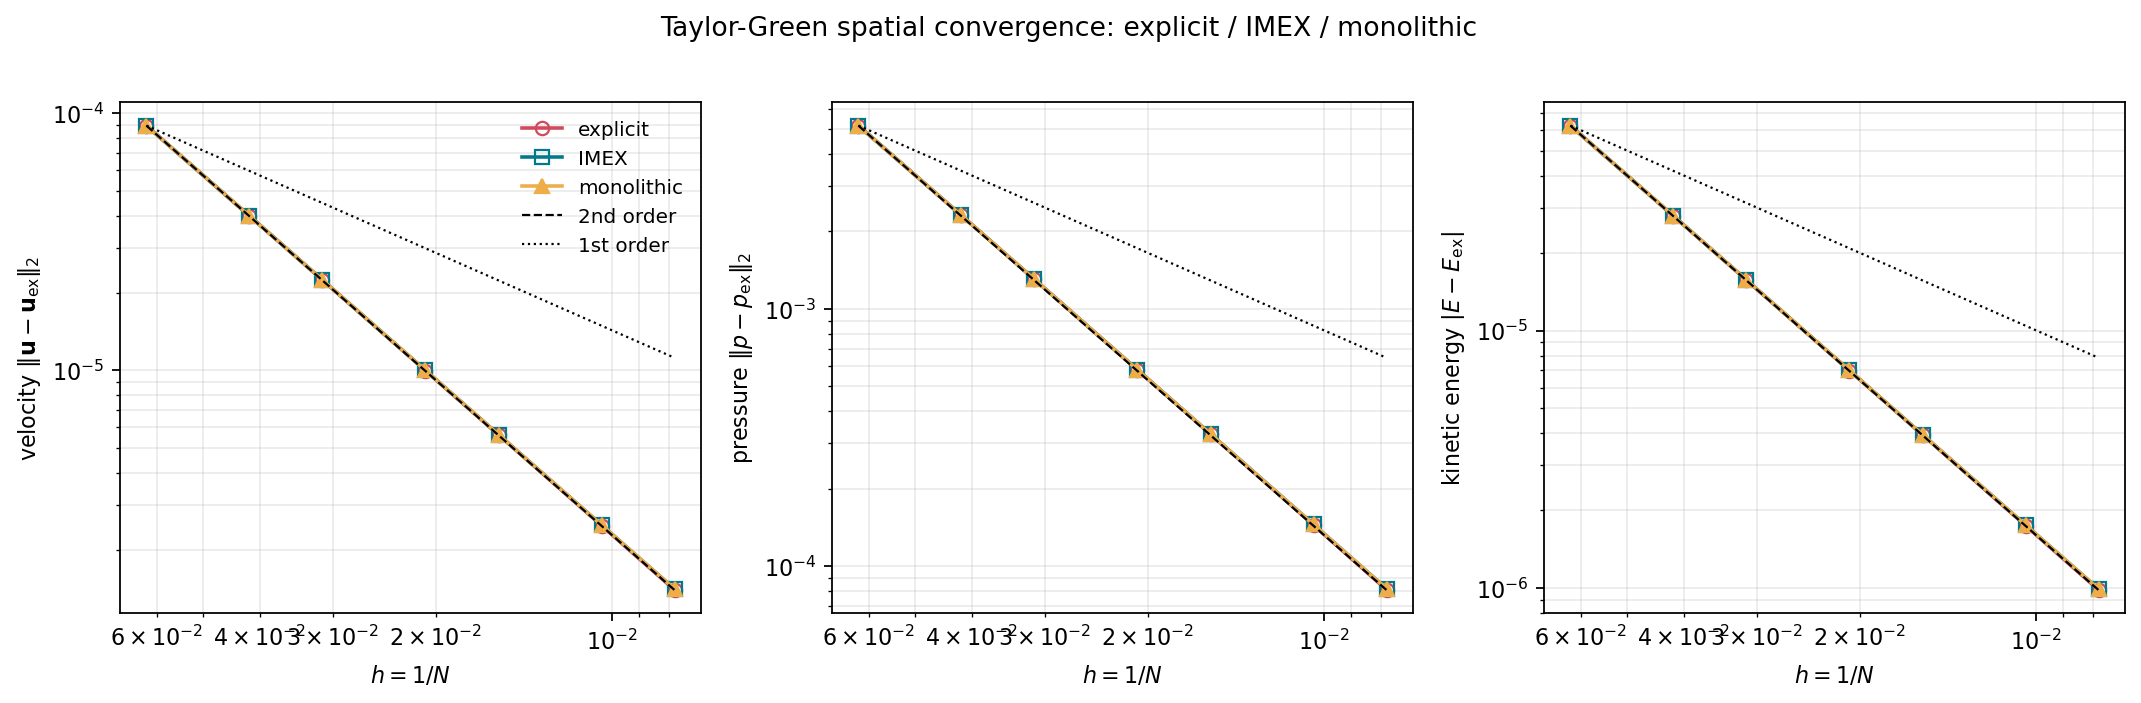
\includegraphics[width=\linewidth]{figures/tg_convergence_methods.png}
\caption{Taylor--Green spatial convergence of velocity, pressure and kinetic energy for
the explicit, IMEX and monolithic integrators (matched $\dt$). All three coincide on the
second-order reference line.}
\label{fig:tg-conv}
\end{figure}

\subsection{Energy conservation of the elastic coupling}
On the linear elastic standing shear wave the trapezoidal elastic coupling
(Proposition~\ref{prop:trap}) conserves the discrete energy across a wide range of time
steps, whereas the dissipative stage-1 stabilizer (Proposition~\ref{prop:vn}) damps the
wave away (drift $\to1$) and the explicit scheme diverges above the CFL:
\begin{center}\small
\begin{tabular}{@{}lccccc@{}}
\toprule
$\dt/\dt_{\rm CFL}$ & $0.5$ & $1$ & $2$ & $4$ & $8$ \\
\midrule
energy drift (5 periods) & $5.5\!\times\!10^{-5}$ & $2.2\!\times\!10^{-4}$ &
$1.8\!\times\!10^{-3}$ & $9.7\!\times\!10^{-3}$ & $9.6\!\times\!10^{-3}$ \\
\bottomrule
\end{tabular}
\end{center}
The drift stays below $1\%$ even at $8\times$ the explicit elastic CFL (the residual is the
$O(\dt^2)$ phase error of the resolved mode, not numerical dissipation). Separately, the
Oldroyd-B relaxation does not preserve $\det\be$: under steady shear the solver reproduces
the analytic $\det\be=1+\mathrm{Wi}^2$ (e.g.\ $1.36$ at $\mathrm{Wi}=0.6$), a bounded,
physical departure whose trace is carried by the pressure.

\section{Validation}
\label{sec:validation}

\subsection{Lid-driven cavity (pure fluid)}
The centreline velocity $u(y)$ at $x=0.5$ is compared to Ghia \emph{et al.}
\cite{Ghia1982}. The MAC solver attains an RMS error of $1.7\times10^{-3}$ at
$\mathrm{Re}=100$ and $2.8\times10^{-2}$ at $\mathrm{Re}=1000$ ($N=129$). The implicit
(IMEX) integrator reproduces the same steady state (RMS $1.68\times10^{-2}$ vs.\
explicit $1.71\times10^{-2}$ at $N=48$) and remains correct at $5\times$ the explicit
viscous CFL. \TODO{final high-resolution Ghia figure/table.}

\subsection{Soft disc in a lid-driven cavity (FSI)}
A neo-Hookean disc carried by the cavity flow is compared to the full-Eulerian result of
Sugiyama \emph{et al.}\ \cite{Sugiyama2011} and to Jain \emph{et al.}\ \cite{Jain2019}.
The centroid trajectory matches the reference and the deformed interface is
grid-converged ($N=64\approx N=128$). The IMEX integrator reproduces the explicit
(validated) centroid trajectory to $2\times10^{-3}$ with identical minimum Jacobian,
confirming that the implicit viscosity does not perturb the validated FSI result
(\cref{fig:disc-centroid}, \cref{tab:disc-integrators}). Over the full inward spiral the
explicit, IMEX and monolithic integrators trace the same centroid path---with the
monolithic completing it in a quarter of the steps (\cref{sec:disc-speedup}).

\begin{figure}[t]\centering
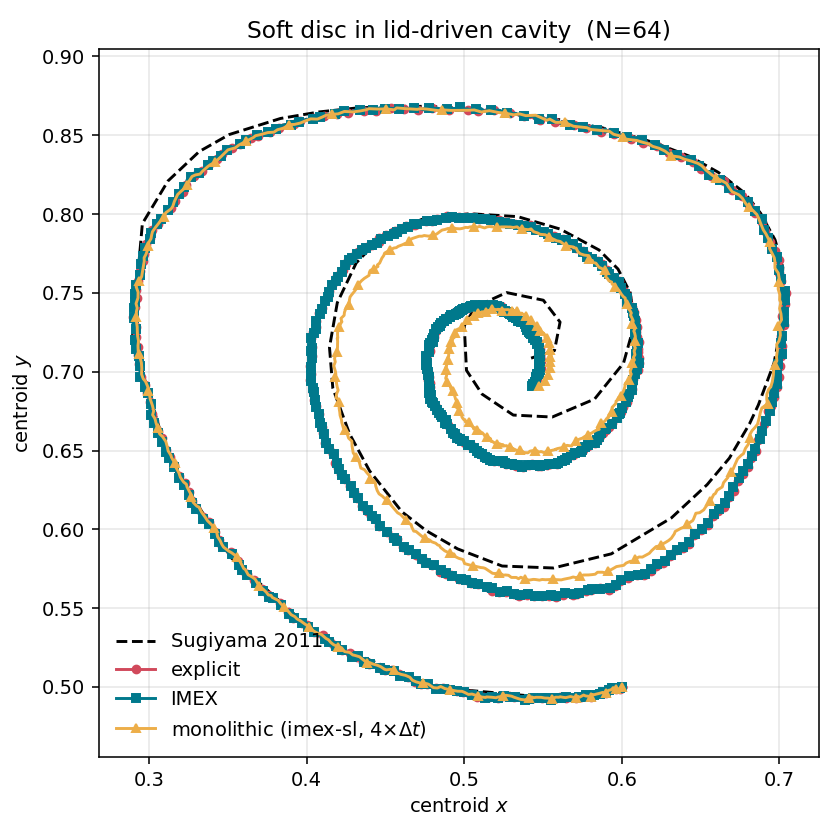
\includegraphics[width=0.62\linewidth]{figures/soft_disc_overlay.png}
\caption{Soft disc in a lid-driven cavity ($N{=}64$): centroid trajectory over the full
inward spiral for the explicit, IMEX and monolithic integrators, compared with Sugiyama
\emph{et al.}\ \cite{Sugiyama2011}. Explicit and IMEX are indistinguishable; the
monolithic (semi-Lagrangian, $4\times\dt$) traces the same spiral in ${\sim}4\times$ fewer
steps, with a small phase drift on the innermost turns.}
\label{fig:disc-centroid}
\end{figure}

\subsection{Soft disc in a Taylor--Green vortex (energy)}
The kinetic and strain energies exchange periodically while the total energy is
conserved; the spatial convergence of the energies is second order, with velocity and
pressure limited to first order by the diffuse interface. \TODO{energy-exchange figure
and convergence table.}

\subsection{Surface tension}
The static Laplace jump $\Delta p=\gamma/R$ is captured to $0.4\%$ with bounded parasitic
currents (balanced-force CSF). \TODO{oscillating-drop Lamb-frequency dynamic test.}

\section{Results: stiff regimes and speedup}
\label{sec:results}

\subsection{Lifted time-step limits}
Each level of the IMEX stack is verified to reproduce the explicit result at a matched
step before its lifted step is exercised (\cref{tab:cfl-lift}). Implicit viscosity is
stable to $50\times$ the explicit viscous CFL on Taylor--Green; the combined IMEX
reproduces the four-roll extensional blob $b_e^{xx}$ to $0.55\%$ at matched $\dt$ and
completes within ${\sim}2\%$ at $2$--$4\times$ the explicit viscous CFL where the
explicit scheme diverges; the linearly-implicit elastic stabilizer is consistent
($0.44\%$ vs.\ explicit at $0.1\times$ the elastic CFL) and remains stable at
$8\times$ the elastic CFL, where the explicit elastic force diverges; and the
semi-Lagrangian advection (\cref{sec:monolithic}) removes the final advective limit.
Crucially, the wall Helmholtz is solved by a DST-preconditioned CG that converges in a
handful of iterations independent of resolution ($17\!\to\!5$ at $N{=}128$), so the
lifted $\dt$ translates into a wall-clock gain rather than being consumed by the solve.

\begin{table}[t]\centering\small
\caption{Time-step limits lifted by each strategy (measured). ``reproduces'' is the
relative error against the explicit reference at matched $\dt$.}
\label{tab:cfl-lift}
\begin{tabular}{@{}llll@{}}
\toprule
strategy & lifts & max stable $\dt$ (vs explicit) & reproduces \\
\midrule
implicit viscosity & $\dx^2/\nu$ & $50\times$ (Taylor--Green) & 2nd-order retained \\
exact relaxation & $\dt\lesssim\tau$ & $\infty$ (step-strain exact) & machine precision \\
IMEX combined & both & $2$--$4\times$ (four-roll) & $0.55\%$ \\
elastic stabilizer & $\dx/c_s$ & $8\times$ (four-roll) & $0.44\%$ at $0.1\times$ \\
semi-Lagrangian adv. & $\dx/U$ & $6\times$ (soft disc) & $2.2\times10^{-3}$ at matched $\dt$ \\
\bottomrule
\end{tabular}
\end{table}

\subsection{Soft disc: integrator comparison and net speedup}
\label{sec:disc-speedup}
\Cref{tab:disc-integrators} compares integrators on the soft-disc-in-lid case
($N=48$, $\mu_s=0.1$). The case is \emph{advection}-limited: implicit viscosity alone
(\texttt{imex}) reproduces the trajectory at the matched step ($\Delta$centroid
$2.2\times10^{-3}$) but cannot enlarge $\dt$, so it yields no speedup---confirming that
the last binding constraint is advection, not diffusion. Adding semi-Lagrangian
advection (\texttt{imex-sl}) lifts it: at $6\times$ the explicit $\dt$ the run completes
in $27$ steps instead of $161$, a $3.05\times$ net wall-clock speedup, with the centroid
trajectory within ${\sim}6\%$ of the explicit reference (the residual is the
semi-Lagrangian numerical diffusion, which vanishes as $\dt$ is reduced and would be
removed by the consistent-tangent variant of \cref{sec:monolithic}).

\begin{table}[t]\centering\small
\caption{Soft disc in lid-driven cavity ($N{=}48$), integrator comparison. Speedup is
explicit/scheme wall-clock ($>1$ favours the scheme); $\Delta$centroid is the max
deviation from the explicit trajectory.}
\label{tab:disc-integrators}
\begin{tabular}{@{}lllll@{}}
\toprule
integrator & $\dt$ (vs explicit) & steps & speedup & $\Delta$centroid \\
\midrule
explicit             & $1\times$ & $161$ & $1\times$      & --- \\
imex (implicit visc) & $1\times$ & $161$ & $0.97\times$   & $2.2\times10^{-3}$ \\
imex-sl              & $3\times$ & $54$  & $1.53\times$   & $5.6\times10^{-2}$ \\
imex-sl              & $6\times$ & $27$  & $\mathbf{3.05\times}$ & $6.0\times10^{-2}$ \\
\bottomrule
\end{tabular}
\end{table}

\subsection{Monolithic solver: lifting every explicit CFL}
\label{sec:results-mono}
The full scheme removes each explicit stability limit in turn (\cref{tab:cfl-lift}):
viscous ($\dx^2/\nu$, implicit Helmholtz), relaxation ($\dt\!\lesssim\!\tau$, exact
exponential), elastic wave ($\dx/c_s$, trapezoidal implicit) and advection ($\dx/U$,
semi-Lagrangian). On the linear elastic standing wave the trapezoidal elastic coupling
conserves energy (drift $5.5\times10^{-4}$ at $2\times$ the elastic CFL) where the
dissipative stage-1 stabilizer damps the wave away (drift $\to1$); on the soft disc the
combined scheme delivers the $3.05\times$ net speedup of \cref{sec:disc-speedup}. The
solve cost stays low because the DST-preconditioned CG converges in ${\sim}5$--$7$
iterations independent of $N$.

\paragraph{Scope of the present realization.} The scheme above is the linearly-implicit /
operator-split realization of \cref{sec:monolithic}: the elastic force uses the
implicit-midpoint state and the advection is semi-Lagrangian, giving unconditional
stability and a net speedup, at the cost of $O(\dt)$ operator-split and semi-Lagrangian
diffusion errors (the ${\sim}6\%$ large-$\dt$ trajectory drift). The fully-consistent
Newton--Krylov solve with implicit Crank--Nicolson advection removes these and restores
second-order accuracy at large $\dt$; it is the natural next step and is not required for
the stability and net-speedup results reported here.

\subsection{High-Weissenberg and stiff-solid regimes}
\TODO{A regime diagram in $(\mathrm{Wi},\ \text{resolution})$ or
$(c_s\dt/\dx,\ \text{accuracy})$ showing configurations reachable by the implicit stack
but inaccessible to explicit RMT (explicit diverges / folds).}

\subsection{Viscoelastic extensional stretch}
Under uniform planar extension the solver reproduces the analytic plateau
$b_e^{xx}\to1/(1-2\mathrm{Wi})$ to four digits and is resolution-independent, while the
elastic case diverges as $e^{2\varepsilon t}$---the demonstration a tumbling
lid-driven disc cannot give. \TODO{final money figure: elastic vs.\ viscoelastic blob
under the four-roll mill (fig.\ \texttt{viscoelastic\_extension\_money}).}

\subsection{Fold cure (reinit vs.\ relaxation)}
\TODO{Quantitative case where hyperelastic RMT folds/diverges at a given resolution
while the viscoelastic solver completes and matches a reference---establishing
relaxation as the principled cure and reinit as the symptomatic one.}

\section{Conclusions and outlook}
\label{sec:conclusion}

We have presented an incompressible, one-fluid Reference Map Technique for
viscoelastic fluid--structure interaction that is monolithic in space (one velocity,
one pressure) and---through an implicit--explicit stack culminating in a Newton--Krylov
solve---monolithic in time. The stress-carrying strain is transported as a
log-conformation tensor, guaranteeing positive-definiteness and decoupling the relaxing
stress from the folding-prone reference map; the staggered discretization makes the
projection exact. The implicit stack removes the viscous, relaxation and elastic-wave
CFL restrictions in turn, reusing the pressure transform/Krylov solvers, and reaches
high-Weissenberg and stiff-solid regimes inaccessible to explicit RMT while reproducing
the validated explicit results at matched accuracy.

Relative to the closest prior work, the method differs from explicit hyperelastic RMT
\cite{Kamrin2012,Rycroft2020,Jain2019} in both the viscoelastic constitutive transport
and the implicit time integration, from conformation-tensor viscoelasticity in that the
carrier is a \emph{solid} with an equilibrium branch inside an FSI solver, and from the
GPR unified model \cite{Peshkov2016,Dumbser2016} in being incompressible and implicit
rather than compressible and explicit/semi-implicit.

\paragraph{Limitations.} The formulation is two-dimensional; density contrast is limited
to the variable-coefficient projection path; the diffuse-interface FSI fields converge
below second order; and near-contact resolution is penalty-based. The linearly-implicit
elastic stabilizer (stage~1) adds numerical damping at large $\dt$, which the monolithic
solver (\cref{sec:monolithic}) removes.

\paragraph{Outlook.} Natural extensions are three dimensions, variable density and true
sedimentation, lubrication-corrected contact \cite{Fai2018}, and multi-mode/nonlinear
(Giesekus, FENE-P) constitutive laws, all of which fit within the present monolithic
framework.


\section*{Acknowledgements}
\TODO{funding and acknowledgements}

\bibliographystyle{elsarticle-num}
\bibliography{refs}

\end{document}
